\documentclass[twoside,a4paper]{report}
\usepackage[T1]{fontenc}
\usepackage[utf8]{inputenc}
\usepackage[english]{babel}
\usepackage{hyperref}
\usepackage[round]{natbib}
\usepackage{float}
\usepackage{ amssymb }
\usepackage{array, makecell}
\usepackage{booktabs, tabularx}
\usepackage{setspace}
\usepackage{graphicx}
\usepackage{mathtools}
\usepackage{titling}
\usepackage{endnotes}
\usepackage{lscape}
\usepackage{verbatim}
\usepackage[labelfont=bf]{caption}
\DeclareMathOperator*{\argmin}{arg\,min}
\DeclareMathOperator*{\argmax}{arg\,max}
\newcolumntype{L}{>{\centering\arraybackslash}m{1.6cm}}
\usepackage[hmarginratio=1:1]{geometry}
\graphicspath{ {./images/} }
\newcommand{\subtitle}[1]{%
	\posttitle{%
		\par\end{center}
	\begin{center}\LARGE#1\end{center}
	\vskip0.5em}%
}

\title{ALBERT LUDWIGS UNIVERISTY OF FREIBURG
\\{\Large MASTER THESIS}}

\subtitle{\line(1,0){250}\\\textbf{\Huge Multisite RNA-RNA Interaction Prediction}\\\line(1,0){250}}	

\author{Yogapriya Ayyanarmoorthy}
\date{\today}

\begin{document}
	
	\maketitle
	
	\tableofcontents
	
	\chapter{Introduction}
	RNA molecules play important roles in various biological processes.Their regulation and function are mediated by interacting with other molecules. 	Forming base pairs between two RNAs, called RNA-RNA interactions (RRI). There are fast and reliable single interaction site (S-RRI) prediction tools like IntaRNA, that often show the additional sites within their suboptimal list, ie. are capable of modelling all sites individually but not in a joint prediction. Many RNAs interact via multiple synchronous, non-overlapping subinteractions (M-RRI), e.g. OxyS-fhlA. The simultaneous prediction of both intra- and inter-molecular base pairing allowing for multiple sites is computationally expensive. Some known approaches are IRIS, piRNA, NUPACK. Here we use a S-RRI prediction tool (namely IntaRNA) for the prediction of M-RRI.
	
	\section{Biological Background of RNA}
	In this thesis, I will focus on Ribonucleic acids (RNA). First of all, I would like to provide the basic biological background that is essential for the thesis. Ribonucleic acid, or RNA is one of the three major biological macromolecules that are important for all known forms of life (along with DNA (deoxyribonucleic acid) and proteins). The "central dogma" of molecular biology states that the flow of genetic information in a cell is from DNA through RNA to proteins: “DNA makes RNA makes protein” (as first suggested by Jean Brachet in 1960 )\citep{brachet1956remarks}. The process by which DNA is copied to RNA is called \textit{transcription}, and that by which RNA is used to produce proteins is called \textit{translation}. RNAs also play an important role in protein synthesis. \\
	
	 DNA is double stranded and RNA is a single-stranded molecule. Each strand of RNA is a sequence of four building blocks called \textit{nucleotides}. Each nucleotide contains Sugar, phosphate and nitrogen containing bases. The sugar and phosphate groups form the backbone of RNA strand and the bases bond to each other.The RNA molecules are represented as a sequence $S \in \{A, C, G, U\} ^*$, where A (adenine), C (cytosine), G (guanine), U (uracil) are the bases of the nucleotide chain.\\
	 
	According to their potential for coding, RNA's are classified into two major categories i.e., coding RNAs and noncoding RNAs. Coding RNAs mostly refers to mRNA that encodes protein to act as different components including cell structures, signal transductors and enzymes. Noncoding RNAs act as cellular regulators with no protein encoding.\\
	Complementary bases $C$-$G$ and $A$-$U$ form stable base pairs with each other using hydrogen bonds. These are called Watson-Crick pairs. Also important are the weaker $U$-$G$ wobble pairs. Together they are called \textit{canonical base pairs}. In general, Isolated base pairs are unstable. If two interacting bases belonging to the same molecule of RNA form \textit{intra-molecular} structures and if they belong to different molecules of RNA form \textit{inter-molecular} structures, as seen in figure ~\ref{fig:secondarystructure}\\
	
	The prediction of RNA-RNA interaction is intended to predict these intermolecular structures between two RNA molecules, an extremely important step in understanding the role of ncRNAs. However, Intra and intermolecular structures are not mutually exclusive.\\
	
	\begin{figure}[h]
	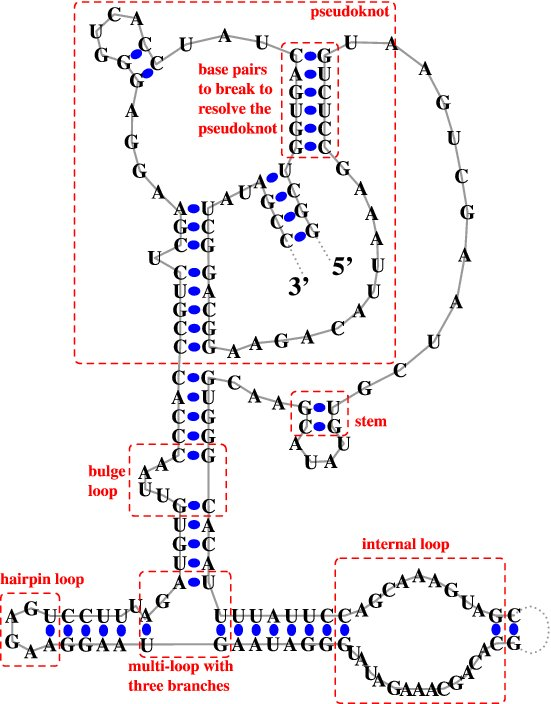
\includegraphics[width=0.7\linewidth]{secondary_structure}
	\centering
	\caption{Schematic representation of the secondary structure (a set of base pairs) for the RNase P RNA molecule of Methanococcus marapaludis from the RNase P Database. Thick blue dots represents base pairs and red dashed boxes represent structural features such as stacking, bulges, hairpin , interior, multi loops and pseduoknot structure. This Figure was taken from the RNAStrand webpage.
	\label{fig:secondarystructure} 
    \citep{andronescu2008rna}}
	\end{figure}

	Single stranded nucleic acid sequences contain many complementary regions that can form double helices when the molecule is folded back onto itself. The resulting pattern of double helical stretches interspersed with loops is called the \textit{Secondary} structure of an RNA.\\
	\section{Formal background of RNA}
	Here in this section, I would like to bring up the formal definitions of ribonucleic acid.
	\subsection{RNA Structure}
	Formally, an RNA secondary structure $P$ of $S$ is a set of base pairs:\\
	\begin{center}
	 $ P \subseteq \{(i, j) | 1 \leq i < j \leq n $, $ Si $ and $Sj$ complementary \},\\
	\end{center}
	where $ n = |S| $ and for all $(i, j) , ( i', j' ) \in  P:$\\
	\begin{center}
	$(i = i' \Leftrightarrow j = j')$ and $ i \neq j'$ \\
	\end{center}

	They are different types of RNA secondary structures they are nested
	and crossing structures. Crossing structures contain pseudo-knots, where two structure parts overlap. Nested structures doesn't have any crossing arcs.\\

	To form a valid secondary structure, the base pairs must satisfy a number of limitations. Let the bases be numbered from 1 to n in a sequence. If the bases are complementary, a base pair may form between positions $i$ and $j$ , and if $|j - i | \geq 4$, since there must usually be at least three unpaired bases in a hairpin loop. Let bases $k$ and $l$ form another allowed pair. The pair $k - l$ is said to be compatible with the pair $i - j$ if the two pairs can be present in a structure simultaneously. Pairs are compatible if they are non-overlapping (e.g. $i<j<k<l$ ) or if one is nested within the other (e.g. $i<k<l<j$ ). The Final case, where the pairs are interlocking (e.g. $i<k<j<l$ ) is called  pseudo-knot.These pairs are assumed to be incompatible with
	most dynamic programs. An allowed secondary structure is a set of base pairs that are all compatible with each other.\\
	
	\subsection{Nested secondary structure}
	Nested secondary structures can be uniquely decomposed into so called loops or secondary structure elements. Depending on the number of enclosed base pairs (BP) and unpaired bases (UB), different types of secondary structure elements are distinguished.They are hairpin loop, stacking, bulge loop, internal loop, multi loop. \\
	Let $S$ be a fixed sequence. Further, let $P$ be an RNA structure for $S$.
	\begin{itemize}
		\item a base pair $( i, j ) \in P$ is a \textit{hairpin} loop if\\
			$	\forall i < i' \leq j' < j : (i', j') \notin P. $

		\item a base pair $( i, j ) \in P$ is a \textit{stacking} if\\
		$(i + 1 , j - 1 ) \in P $
		\item two base pairs $ (i, j) \in P$ and $(i' ,j' ) \in P$ form  an \textit{internal} loop $(i,j,i',j')$ if \\
		$i < i' < j' < j $ ; $ (i' - i)+( j - j') > 2$ ; no base pair $(k,l)$ between $(i, j)$ and $(i',j')$
		\item An internal loop is called left (right, resp.) \textit{bulge} if\\
		$ j = j' +1 $ or $ i' = i+1$
		\item A k-\textit{multiloop} consists of multiple base pairs, $(i_1,j_1)$... $(i_k,j_k) \in P$ with a closing base pair $(j_0, i_{k+1}) \in P$ with the property that \\
		$\forall 0 \leq l \leq k : ( j_l < i_{l'+1})$ ; $\forall 0 \leq l , l' \leq k$ is true that there is no base pair $(i' ,j') \in P$ with $i' \in [j_l...i_{l+1}]$ and $j' \in [j'_l...i_{l'+1}]$ .
		\item $(i_1,j_1)...(i_k, j_k)$ are called the \textit{helices} of the multiloop.\\
 	\end{itemize}
 
 
 	 \citeauthor{DeVoe1962TheSO} discovered that vertical stacking of bases gives largest contribution to the stability of the RNA helix. The stacking of unpaired bases is less predictable and stable than the paired bases. Hence, the directly neighboured bases must be taken into account while estimating the energy contribution of a  base pair, that results in the \textit{Nearest Neighbor Model} \citep{borer1974stability}.\\
 	 
 	 \subsection{Nearest neighbor model and energy contributions }
 	 
 	 The Nearest Neighbor Model enables the calculation of a free energy estimate for a given RNA secondary structure. For the performance of work, the free energy can be taken as the amount of energy stored in a system. The positive energy is in the form of heat  and the negative energy is used to destroy the system. Always, lower the energy gives more stable the system. Hence, for the \textit{most stable structure} of RNA , we go for \textit{minimum free energy (MFE)}. The energy difference between the reference state to the system is measured. We have a reference system which we use to understand the stability of the system. ie., $ E(\phi) =0 $. Hence , we need to check not only the hydrogen bonds but also the stacking stability.The Nearest Neighbor Model uses a loop-based structure decomposition. To avoid the duplication of stacking, only inner stacking are taken into account. \\
 	 
 	 \textit{The terminal mismatch} consists of the first unpaired bases immediately after the stacking. The identity of the terminal mismatch provides the energy of the loop. In Bulge or Internal loop also we have the same energy contribution. Energy contributions for external base pairs, which are not enclosed by any other base pairs, are referred to as textit{dangling end contributions}.\\ 
 	 The energy $E(P)$ ~\ref{eq:1} of a nested secondary structure $P$ can be estimated by the sum of loop contributions (see Figure ~\ref{fig:energycontribution})\\
 	 
 	 \begin{equation}
 	 \label{eq:1}
 	 E(P) = \sum_{(i,j) \in P} \begin{cases}
 	 e^H(i,j) & : \text{if hairpin loop}, \\
 	 e^{SBI}(i,j,k,l) & : \text{if stack/bulge/internal loop} ,\\
 	 e^M(i,j,x,x') & : \text{if Multi loop},
 	 \end{cases}
 	 \end{equation}
 	 
 	 Where $e^H$, $e^{SBI}$ and $e^M$ tells the context sensitive energy contributions of the loops. Where $(k,l)$ represents the enclosed base pair of stack,bulge or internal and $x$ represents the unpaired bases and $x'$ represents the helices enclosed in the multi loop. We can see that there is an exponential number of possible multi loop composition. The energy for them can be calculated as below \\
 	 \begin{center}
 	 $e^M(i,j,x,x')= e^M_a+e^M_bx+e^M_cx'$\\
 	\end{center}
 	 where the pseudo energy parameter $e^M_a$ scores the multi loop closing base pair $(i,j)$ , $e^M_b$ represents the penalty for directly enclosed unpaired bases $x$ and $e^M_c$ represents the number of enclosed helices $x'$.
 	 Thus the nearest neighbor model gives the energy contributions for the loop types. \\
 	 
 	 \begin{figure}[h]
 	 	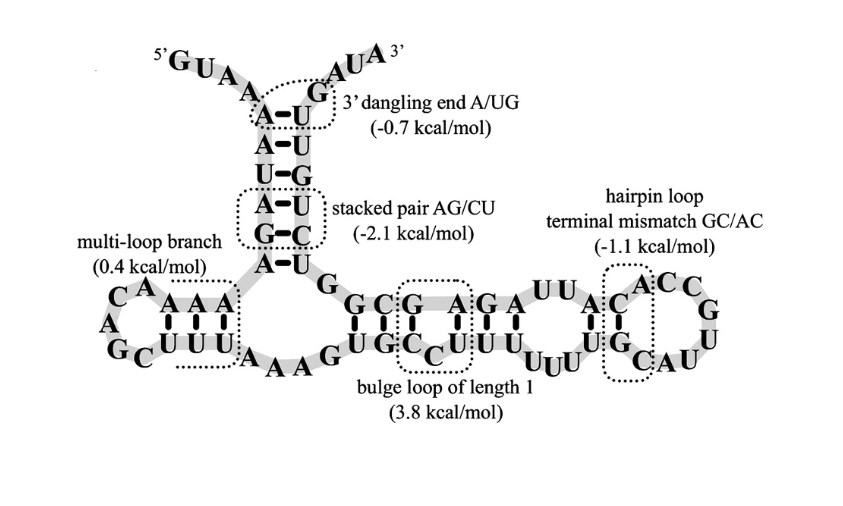
\includegraphics[width=0.9\linewidth]{energy}
 	 	\centering
 	 	\caption{Energy contributions of loops. \citep{andronescu2010computational}}
 	 	\label{fig:energycontribution}
 	 \end{figure}
 	 
 	 
 	 From the above energy model, We can define a recursive dynamic programming algorithm to compute the structure which minimizes the energy function,this is called minimum free energy (mfe) structure. This algorithm was introduced by \citep{zuker1981optimal}.\\
 	 
 	 The basic substructures of the secondary structure of the RNA sequence (i.e., stack, hairpin, internal and multi loop) are independent of each other and the energy of the secondary structure is assumed to be the sum of the energies of the substructure. The algorithm is executed in two steps with a single RNA sequence as input. Firstly, the minimum free energy of the input RNA sequences has been calculated , then traceback is used to recover the secondary structure with the base pairs. Thus given an RNA sequence $S$, Zuker’s algorithm predicts the non-crossing, minimal energy structure $P$ of $S$ in $O(n^3)$ time and $O(n^2)$ space.\\
 	 
 	 \subsection{Structure probabilities and McCaskill algorithm}
 	 Let's discuss about the structural information in terms of probabilities. According to the principal of maximum entropy \citep{jaynes1957information} the best probability distribution for the calculation of the structure or base pair probability is the \textit{Boltzmann Distribution}. These probabilities are calculated according to the Boltzmann weight. For RNA structures the unit of the energy value is $\frac{kcal}{mol}$ or $\frac{J}{mol}$. The RNA structure energy is been rescaled for boltzmann weight computation. i.e., We replace boltzmann constant $k_B$ with "mol-scaled" gas constant $R$\\
 	 
 	 \begin{center}	 
 	 \[ 
 	 w(P)= exp\left( \frac{-E(P)}{RT} \right)
 	 \]
 	 \end{center}
 	 
 	 Where $E(P)$ represents the state energy , $R $ represents the gas constant and $T$ is the temperature.\\
 	 The partition function $Z$ can be calculated using the Boltzmann weights. $Z$ is the sum of the Boltzmann weights of all states within $P$. \\
 	 \begin{center}	 
 	 	\[ 
 	 	Z= \sum_{P \in \mathcal{P}} w(P)
 	 	\]
 	 \end{center}
 	 
 	 $Z$ is used for the calculation of structure and base pair probabilities. So in the total sum, the distribution does not change from a macroscopic point of view,therefore thermodynamic balance is reached.\\
 	 The probability of an RNA structure $P$ is given by \\  
 	  \begin{center}	 
 	 	\[ 
 	 Pr[P|\mathcal{P}] = \frac{w(P)}{Z} 
 	 	\]
 	 \end{center}
  	 and normalising with the partition function $Z$ for the structure ensemble $\mathcal{P}$.  \\
  	
  	 We can also calculate the probabilities of unpaired regions. Formally, we will identify the probability of the subsequences i..j to be unpaired by $Pr_u[i,j]$. This probability depends on  on the whole ensemble of structures that can be formed by the RNA molecule of interest. Thus, it can be computed by\\
     \begin{center}	 
     	\[ 
     	Pr_u[i,j] = \frac{Z^u_{i_j}}{Z}
     	\]
     \end{center}
 	 where $Z^u_{i_j}$ is the partition function of all structures where the subsequence i..j is unpaired.\\
 	 
 	 i.e., 
 	 \begin{center}	 
 	 	\[ 
 	 	Z^u_{i_j}= \sum_{P \subset \mathcal{P}^u_{i_j}} w(P) = Z(\mathcal{P}^u_{i_j})
 	 	\]
 	 \end{center}
  
  	 where $\mathcal{P}^u_{i_j}$ is the ensemble of all structures that are unpaired between i and j.\\
  	 
  	  i.e., 
  	 \begin{center}	 
  	 
  	 	$\mathcal{P}^u_{i_j}$= $\{P \mid \nexists (k,l) \in P\ : i \leq k \leq j $ or $ i \leq l \leq j\}\subseteq \mathcal {P}_{all}$,
  	 
  	 \end{center}
  	 
  	 Where $\mathcal {P}_{all}$ is the ensemble of all structures that can be formed from a sequence. The calculation of accessibility of single stranded regions is carried out using  unpaired probability \citep{muckstein2006thermodynamics}, hence it is very important. 
  
 	 The below figure ~\ref{fig:unpaired} was inspired by the lecture material of RNA bioinformatics lecture .\\
 	 
 	 \begin{figure}[H]
 	 	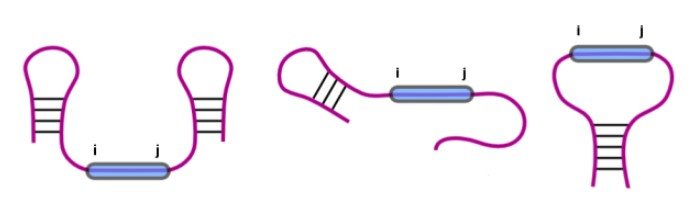
\includegraphics[width=0.8\linewidth]{unpaired}
 	 	\centering
 	 	\caption{Examplary structures that are unpaired in the subsequence i..j.}
 	 	\label{fig:unpaired}
 	 \end{figure}
  
 	 Different probabilities can be calculated using McCaskill algorithm. The McCaskill algorithm \citep{mccaskill1990equilibrium} is used to calculate the partition function $Z$ for a given sequence $S$, which can be used to compute probabilities. It enables efficient computing of the probabilities of the structure of the RNA as well as the probability that a certain base pair is formed. In addition, unpaired probabilities for subsequences can be calculated that reflect the accessibility of RNA parts for other interactions.\\ 
 	
	
	\section{RNA-RNA Interaction}
 	The interaction of RNA molecules is an essential factor for regulatory processes in all organisms. Computational prediction of RNA-RNA interactions (RRI) is a central methodology for the specific investigation of inter-molecular RNA interactions and regulatory effects of non-coding RNAs. RNA–RNA interactions are fast emerging as a major functional component in many newly discovered non-coding RNAs. They are important in many basic cellular activities including transcription, RNA processing, localization, and translation. Interacting RNA strands is classified into two types. ie., Intermolecular and Intramolecular. Many RNA species function is guided by their structure, which is defined by intramolecular base pair formation. Small prokaryotic RNAs display evolutionary unstructured regions that control the expression of their target mRNAs by intermolecular base pairing \citep{wright2013comparative}. Hence, The prediction of both functional intramolecular and intermolecular RNAs are important bioinformatics tasks. \\
 	
 	Let's see about some simple RNA-RNA interactions. In \textit{splicing} , small nuclear RNA's (snRNA) can recognize intronic regions of precursor messenger RNAs(mRNA) which is the important step in identifying the RNA splicing products \citep{modrek2002genomic}. In \textit{translation} transfer RNAs(tRNA) interact with messenger RNAs(mRNA) by reading the three letter code and define amino acid sequence \citep{selmer2006structure}, \citep{ibba2000aminoacyl}. In RNA modification, small nucleolar RNAs(snoRNA) guide the modification of ribosomal RNAs(rRNA) \citep{kiss2002small}. In microRNA (miRNA) targetting, the base pairing between an miRNA and mRNA leads to degradation or translation inhibition of the mRNA \citep{bartel2004micrornas}. For RNA function and regulation these examples gives us the importance of the RNA-RNA interaction. \\
 		
 	In order to allow highly accurate predictions, state-of-the-art methods not only take into account the stability (energy) of possible RNA–RNA interactions, but they also take the accessibility of the interacting subsequences \citep{umu2017comprehensive}.\\
 	
 	\subsection{Formal background of RNA-RNA interactions}
 	Here, we will see the formal background of RNA-RNA interactions.\\
 	In general RNA–RNA interaction prediction (RIP) problem, given two RNA sequences $S^1$ and $S^2$ (e.g., an antisense RNA and its target), the RIP problem asks one to predict their joint secondary structure. A joint secondary structure between $S^1$ and $S^2$ is a set of “pairings” where each nucleotide of $S^1$ and $S^2$ is paired with at most one other nucleotide, either from $S^1$ or $S^2$ \citep{alkan2006rna}.  \\
 	
 	The RNA-RNA interaction is the combination of the set all of all base pairs in $S^1$ , set of all base pairs in $S^2$ and the total intermolecular base pairs between two sequences. Formally, the RRI can be modelled as RRI = $ \uplus $ bp ($S^1$) $ \cup $ $\uplus$ bp ($S^2$) $\cup$ $\uplus$ ($Inter$). Basically, the set of all base pairs of $S^1$ is $P^1$ and $S^2$ is $P^2$ , then $Inter$ is $I$ which denotes the set of all intermolecular base pairs. \\
 	
 		\begin{center}
 		RRI =  $P^1$ $ \cup $  $P^2$ $\cup$ $I$
 		\end{center}
 
	 	\begin{figure}[H]
		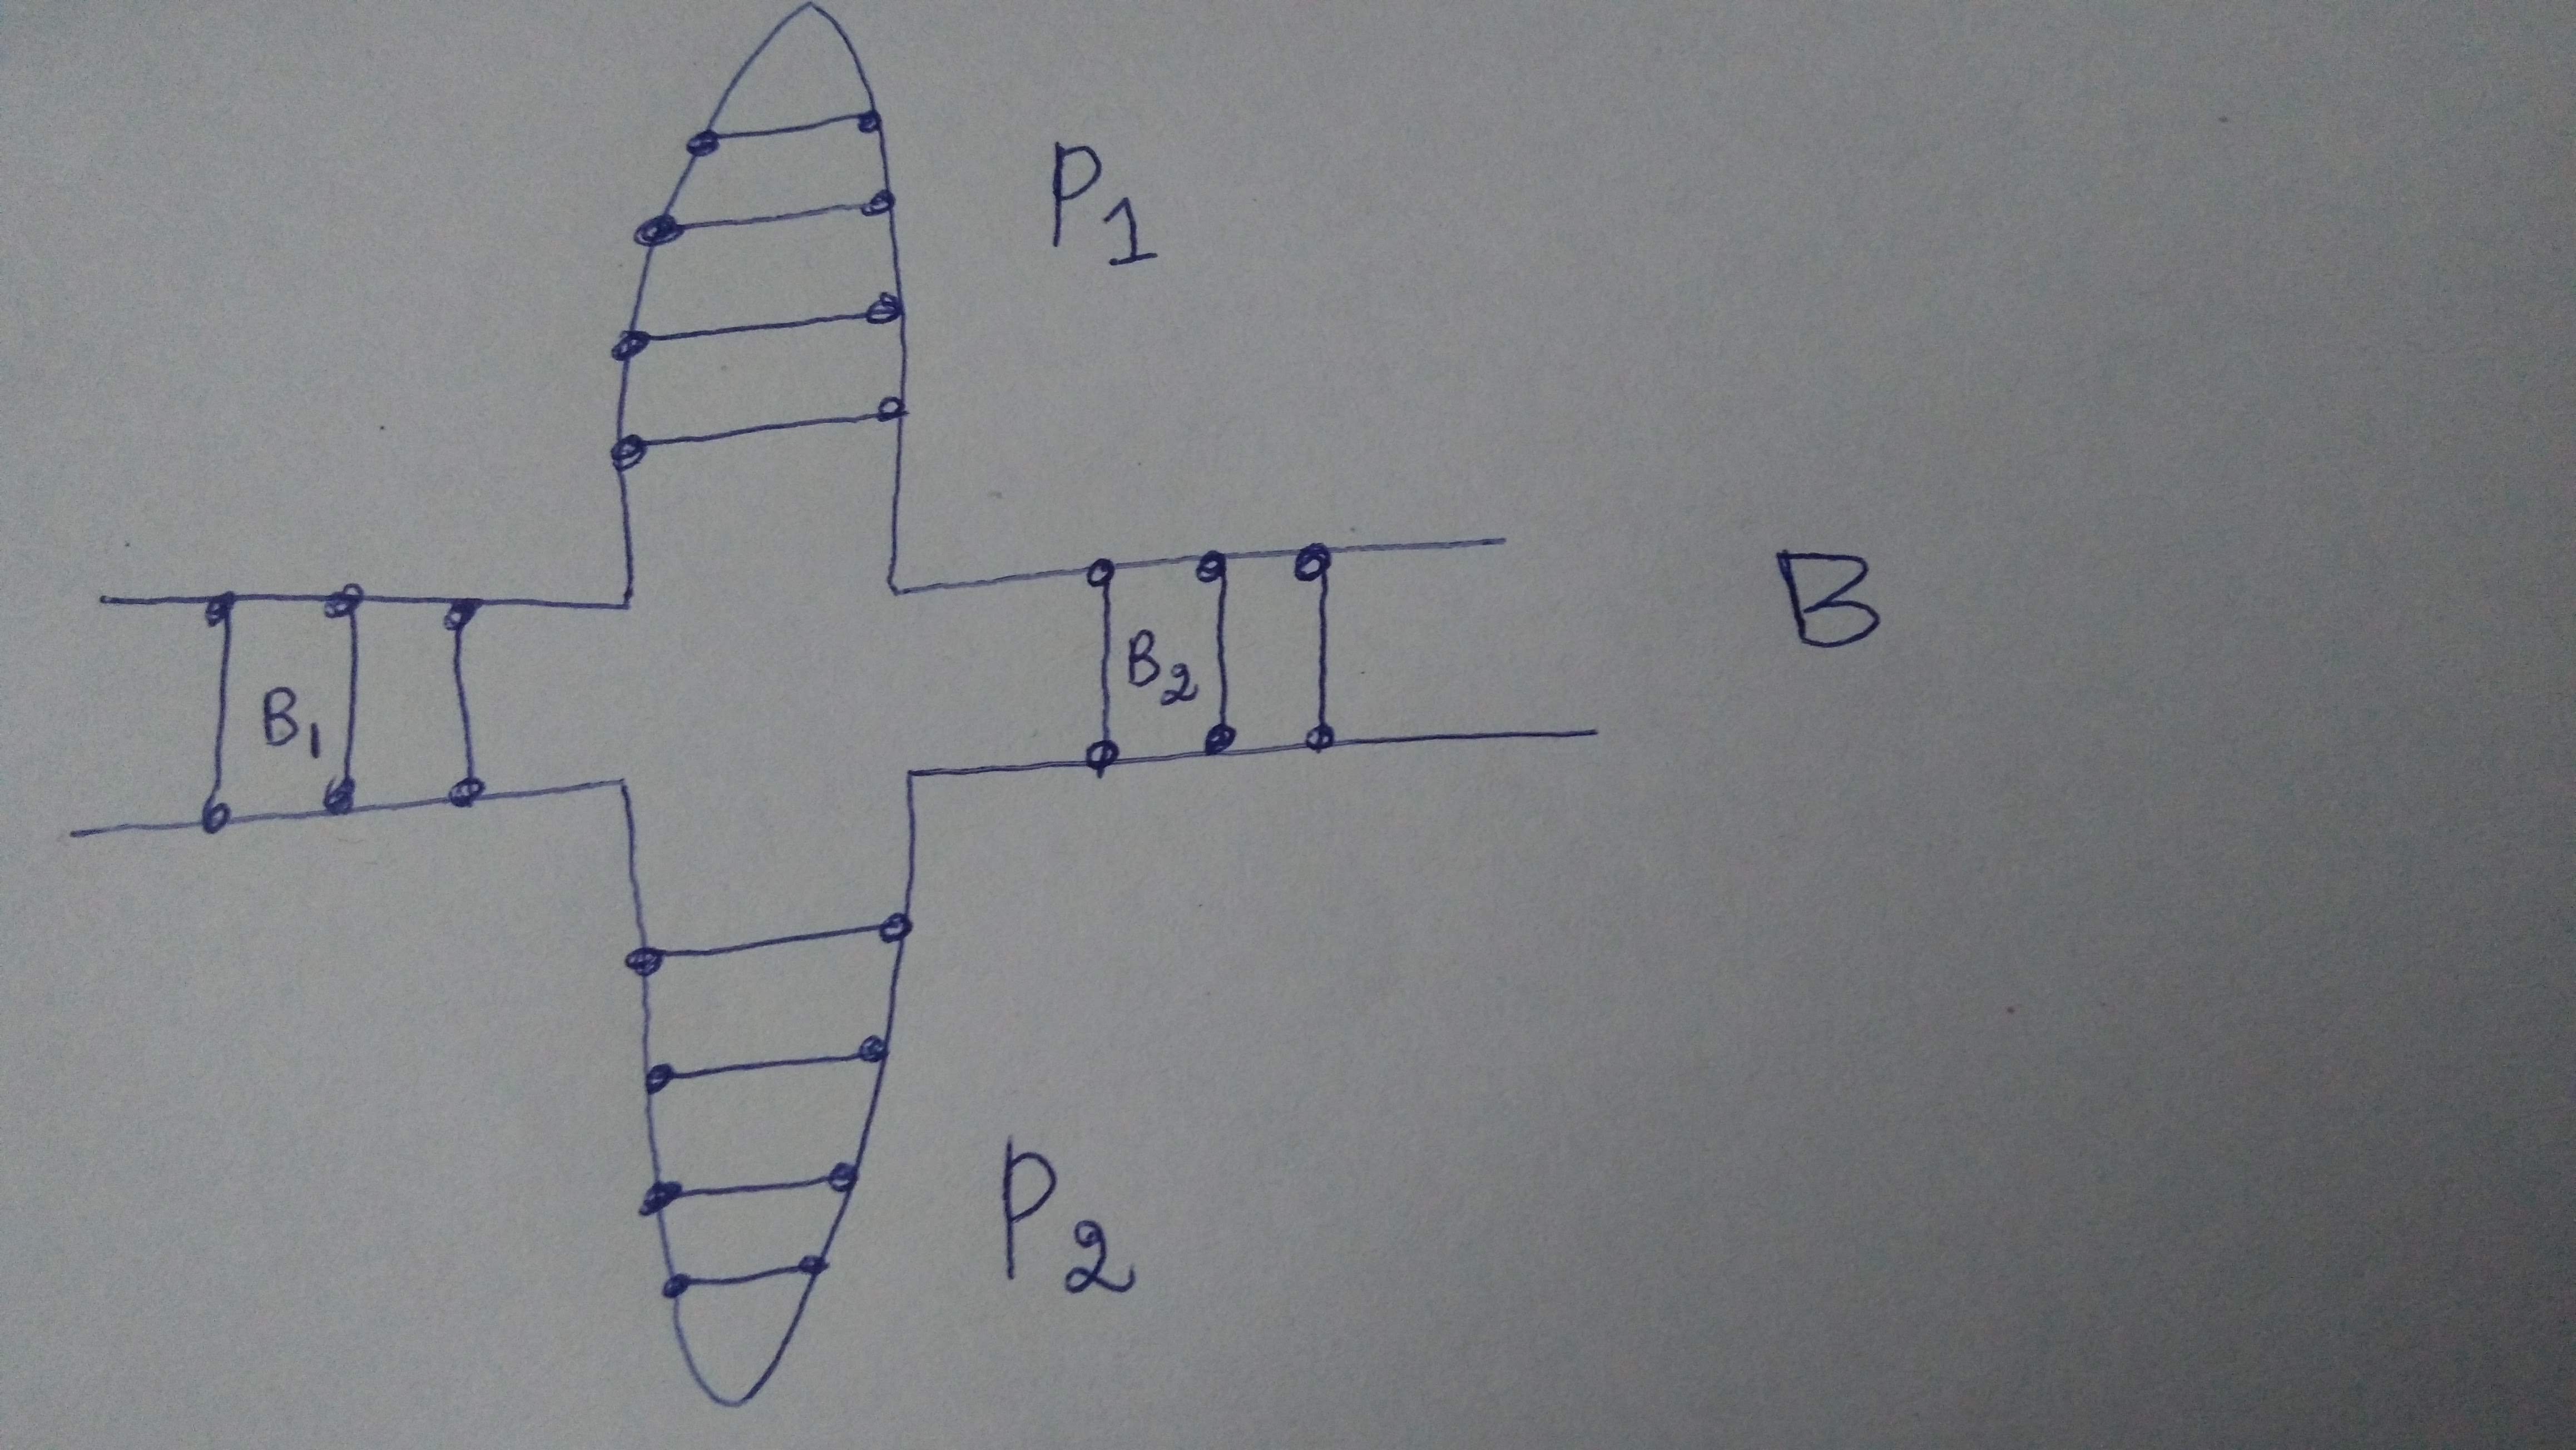
\includegraphics[width=0.6\linewidth]{RRI2}
		\centering
		\caption{Diagrammatic representation of formal RRI }
		\label{fig:RRI2}
	\end{figure}
	
 	In the figure, sky blue colour represents the intramolecular loop with the intermolecular base pairs paired. We will need to find out, how to score them. Here,without further knowledge or energy parameters, we score it via standard loop scores ignoring the intermolecular pairings. The problem starts with the pseudoknot, in the loops where the positions are not paired within the loop ~\ref{fig:position}.\\
 	
 		\begin{figure}[H]
 		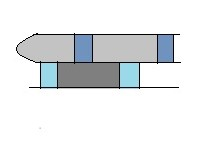
\includegraphics[width=0.5\linewidth]{position}
 		\centering
 		\caption{Positions are not paired within the loop }
 		\label{fig:position}
 	\end{figure}
 	
 	The same problem we have for the scoring of crossing structure in a pseudoknot.\\
 	
 		\begin{figure}[H]
 		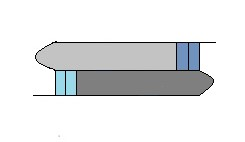
\includegraphics[width=0.5\linewidth]{pseduknot}
 		\centering
 		\caption{Diagrammatic representation of Pseudoknot }
 		\label{fig:pseduknot}
 	\end{figure}
 	
 	
    Now, we further decompose $I$ into the sequence of subsets of consecutive base pairs that form interaction blocks $B$ which is depicted in the figure ~\ref{fig:RRI2} , Where $ I = (B_1 ,..., B_x)$. A block $B$ is the interaction block or interaction site.
 	
 
 
 	\begin{figure}[H]
 		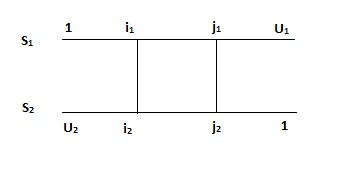
\includegraphics[width=0.6\linewidth]{RRI}
 		\centering
 		\caption{The model for RRI }
 		\label{fig:RRI}
 	\end{figure}
 
 	Further, the interaction block or interaction site "B" can be represented as,
 	
 	\begin{center}
 	 $B = \{ (i_1 , i_2)  \mid  S^1_{i_1}$ complementary to $ S^2_{i_2} \} \subseteq [ 1, n_1] * [1 , n_2] $
 	\end{center}
 	
 	Where for all $(i_1 ,i_2) ,(j_1, j_2) $ is 
 	
 	\begin{center}
 		$(i_1 < i_2) \iff  (j_1 > j_2)$
 	\end{center}
 	
 	ie., It should be non-crossing and no intra molecular base pairs in block region R(B) of $P^1 , P^2$. The block region R(B) is $(i(B) , j(B))$ ie., left and right most base pairs of B concerning $S^1$, where\\
 	
 	\begin{equation*}
 		i(B) = \argmin_{i = (i_1, i_2 ) \in B } (i_1)
 	\end{equation*}
 
 	\begin{equation*}
 			j(B) = \argmax_{i = (i_1, i_2 ) \in B} (i_1)
 	\end{equation*}
 	
 	\begin{figure}[H]
 		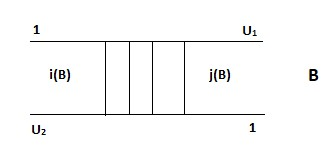
\includegraphics[width=0.6\linewidth]{region}
 		\centering
 		\caption{The model for block region }
 		\label{fig:region}
 	\end{figure}
 	
 	For a valid RRI, lets consider bases $k$ and $l$ form another allowed base pair. Then,
 	
 	\begin{center}
 		 $\forall_{B\in I } :\nexists_{(k,l) \in P^1} : i(B)_1 \le k \le j(B)_1  \wedge   i(B)_1 \le l \le j(B)_1 $ \\$\wedge $\\ 	$\nexists_{(k',l') \in P^1} : i(B)_2 \le k' \le j(B)_2  \wedge  i(B)_2 \le l' \le j(B)_2 $
 	\end{center}
 	
 	where I is the union of all blocks (ie., all inter molecular base pairs)
 	We compute the joint structure between S1 and S2 through minimizing their total free energy. Now, lets see the formal definition of energy of RRI. By using the above RRI equation, we can write energy of RRI as \\
	
	\begin{center}
		$E(RRI) = E(P^1)+E(P^2)+E_init+ \sum_{B_i \in I}E(B_i) + \sum_{B_i \in I} E^{right}_{gap} (B_i,Bi+1, P^1, P^2)$ 
	\end{center}
	
	\begin{figure}[H]
		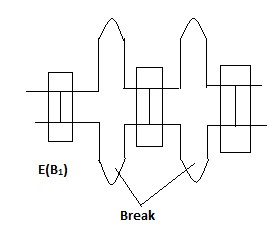
\includegraphics[width=0.6\linewidth]{ene}
		\centering
		\caption{The model for energy of interaction. }
		\label{fig:ene}
	\end{figure}

	The E(I) can be calculated as follows,
	
	\begin{center}
		$E(I) = E(  \uplus  B) + E_{init} $
	\end{center}
	\begin{center}
		where, E( $ \uplus $ B) = $\sum_B$ E(B) + E(break) and $E_{init}$ is fixed init score if I $\neq$ $\phi$ 
	\end{center}
		
	The Energy for the block E(B) can be calculated as  ,
	
	\begin{equation*}
	E(B) =  \sum_{\substack{i \in B \\ j \in B \\ \exists i < j}}E^{SBI}(i,j,k,l)
	\end{equation*}	
	
	where $j = argmin_{i' \in B \wedge i'>i}(i'_1)$
	and for the E(break) it depends on the prediction model which is a tricky part and that will be discussed with the next section along with the approaches idea.\\
	
	
	\section{RNA-RNA Interaction Prediction Approaches}
	There are several available methods, that can be classified according to their underlying prediction strategies, each implicating unique capabilities and restrictions often not transparent to the non-expert user.\\ 
	Mostly for RNA-RNA interaction prediction methods are based on thermodynamic models and provide an efficient computation since Richard Bellman’s principle of optimality \citep{raden2018interactive} can be applied. RNA–RNA interaction prediction approaches are classified according to their algorithmic idea into hybrid-only interaction prediction,General interaction prediction, concatenation-based/cofolding interaction prediction , and accessibility-based interaction prediction. \\
	In the following subsections we will see about the approaches used for predicting the RNA-RNA interactions.\\

	
	\subsection{Hybrid}
	In hybrid-only interaction approach, the identification of RNA-RNA interaction doesn't consider intramolecular base pairs ~\ref{fig:rnahybrid} and they can be done with $O(nm)$ time and space complexity for two RNA sequences $S1$, $S2$ of lengths $n$ and $m$ respectively \citep{tjaden2006target}.\\
	
	\begin{figure}[H]
		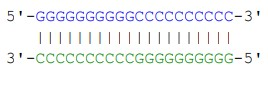
\includegraphics[width=0.4\linewidth]{rnahybrid}
		\centering
		\caption{ A full duplex structure where no intramolecular base pairs are assumed. The figure is taken from the paper \citep{wright2018structure}} 
		\label{fig:rnahybrid}
	\end{figure}
	
	
	 A dynamic programming approach using a simplified energy model with two dimensional table H is filled via the prefix-based recursion ~\ref{eq:2} for the nussinov like interaction prediction.\\
	 \begin{equation}
	 \label{eq:2}
	H_{ij} = max \begin{cases}
	H_{i-1,j-1}+1 & : \text{if $S^1_i$, $\overleftarrow{S^2_j}$ are compl. base pair }, \\
	H_{i-1,j} \\
	H_{i,j-1} ,
	\end{cases}
	\end{equation}
	Where $H_{ij}$ is the maximal number of intermolecular base pairs for the prefixes $S^1_1..i$	and $\overleftarrow{S^2_1..j}$ the reverse sequnce of $S^2$. The visual representation of the recursion scheme ~\ref{fig:hybrid} . The above equation is the s a variant of the global sequence alignment approach by \citep{needleman1970general} using scoring scheme i.e.,base pair instead of match/mismatch scoring for$S^1_i$, $\overleftarrow{S^2_j}$ no gap cost. Hence , when initialising $ H_{i,0} / H_{0,j} $ with 0, the $H_{n,m} $ gives the maximal number of intermolecular base pairs and we can trace back them. As stated above, this approach has very low runtime.\\
	 \begin{figure}[h]
		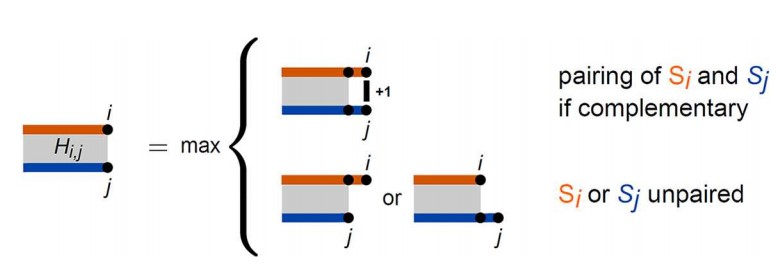
\includegraphics[width=0.8\linewidth]{hybrid}
		\centering
		\caption{Recursion scheme to maximize intermolecular base pairs between two RNAs $S1$ and $S2$ represented in orange/blue, respectively} 
		\label{fig:hybrid}
	\end{figure}
	The energy for RRI can be calculated as follows:
	\begin{equation*}
		E(break) = \sum _{\substack {B_i \in I}} E_{loop}(j(B_i),i(B_{i+1}))
	\end{equation*}
	They are implemented in tools like TargetRNA, RNAhybrid, RNAplex. The main advantages of this approach is they allows temperature to taken into account, they are very fast and easy to calculate the significance of hits.  Since,  intramolecular base pairing is ignored they are used for the identification of short RNA's and overestimate the length of target sites. These disadvantages can be overcome by concatenation and accessibility based approaches.\\ 
	
	\subsection{General}
	One of the most common general approach that is used for predicting the two intermolecular RNA molecules is IRIS \citep{pervouchine2004iris} method. This method is basically implemented by dynamic programming where it is the product of the sequence alignment and two MFOLD type secondary structure prediction algorithms. They can predict \textit{general duplex structures}. This method is applied to some well known interactions such as OxyS with fhlA mRNA which basically forms a double kissing hairpin interactions as shown in below fig ~\ref{fig:doublekiss}.It uses the energy model where the number of base pairs can be maximised.\\
	
	 \begin{figure}[H]
		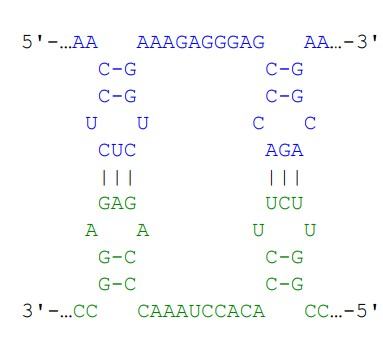
\includegraphics[width=0.4\linewidth]{doublekiss}
		\centering
		\caption{ Double kissing hairpin interaction. The blue and green denotes the first and second sequnence of RNA. Base pairs are denoted by dash. The picture is taken from the paper } 
		\citep{wright2018structure}
		\label{fig:doublekiss}
	\end{figure}
	
	In IRIS method we use nussinov recursion matrix for computing the base pair maximization without intermolecular interactions. let's represent $N^{R^1}$ , $N^{R^2}$ denotes the interacting RNA's $R^1$ and $R^2$. The recursion matrix $M^{i, k}_{j, l}$ denotes the maximal number of both intramolecular and intermolecular base pairs for the interacting subsequences $ R^1_{i..k}$, $R^2_{j..l}$. The recursion ~\ref{eq:3} is as follows    \\ 
	
	 \begin{equation}
	 \label{eq:3}
	M^{i..k}_{j..l} = \max \begin{cases}
	0 & : \text{if both $j > l $  and $ i > k $}, \\
	N^{R^1_{i,k}} , N^{R^2_{j,l}} & : \text{no interaction considered if $j > l $  and $ i > k $} \\
	M^{i+1..k-1}_{j..l}+1 , M^{i..k}_{j+1..l-1}+1 & : \text{intramolecular base pair if $R^1_i, R^1_k $  or $ R^2_j , R^2_l$ can pair}  \\
	M^{i+1..k}_{j+1..l}+1 , M^{i..k-1}_{j..l-1}+1 & : \text{intermolecular base pair if $R^1_i, R^2_j $  or $ R^1_k , R^2_l$ can pair} \\
	\max_{s,t} \{ 
	M^{i..s}_{j..t} + 	M^{s+1..k}_{t+1..l} \} & : \text{ decomposition of interaction site}\\
	\end{cases}
	\end{equation}
	
	In the above recursion the $j > l $  and $ i > k $ represents the individual structure formation of $R^1$ and $R^2$ and are given by $N^{R^1}$ , $N^{R^2}$ . In third case, we omit omits the minimal intramolecular base pair span $s_l$ for the simplicity purpose. The last case is does not account for generalized pseudoknots. The fig ~\ref{fig:iris} shows the visual depiction of the recursion. For treating the generalized pseudoknots, we need to replace it with $max \{ M^{i..s}_{k..t} + 	M^{s..j}_{t..l} , M^{i..s}_{t..l} + 	M^{s..j}_{k..t}\}$. After examining this interaction, it was found that the fact it is not the minimum free energy structure.\\
	
	\begin{figure}[H]
		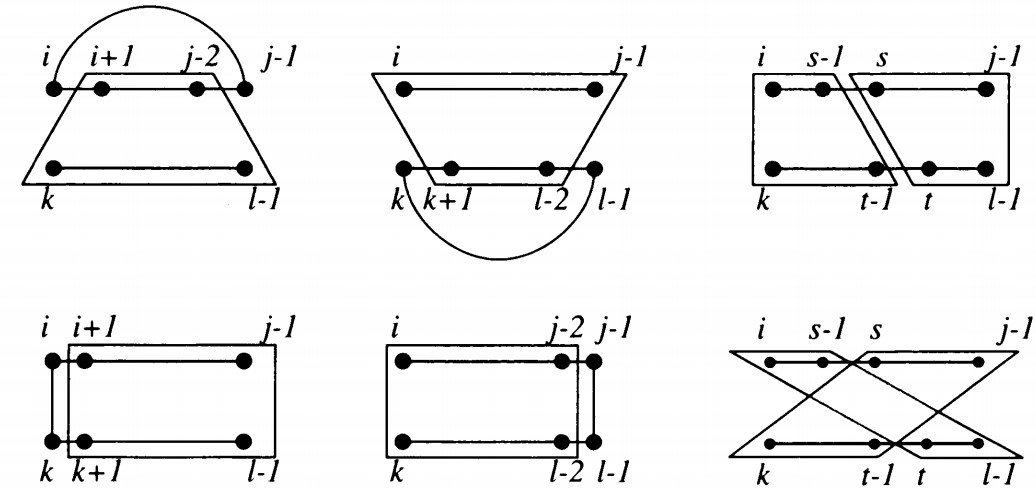
\includegraphics[width=1.0\linewidth]{iris}
		\centering
		\caption{ Depiction of the recursion $M^{i..k}_{j..l}$. Figure is taken from the paper} 
		\citep{wright2018structure}
		\label{fig:iris}
	\end{figure}
	

	The time and space usage of IRIS are $ O(n^6)$ and $ O(n^4)$, respectively. The partition function version of RNA-RNA interaction prediction allows to predict the suboptimal interaction and its probabilities also the computation of probabilities of intermolecular interactions, which is used to access the stability. Due to its high complexity, several approaches for reducing the requirements of this method have been introduced.\\
	
	 
	\subsection{Concatenation}
	Concatenation or co-folding approach is used for predicting the interacting base pairs of two RNA molecules. Two or more sequences are concatenated  into a single sequence with special inter-spacing linker sequences. The final sequence is used within an adaptation of a standard structure prediction that takes  care of the linker sequences. The first implementation of this approach was by using Nearest neighbor model which was used for mfold and then implemented in tools like MutliRNAfold and RNAcofold.\\
	
	This is extension of nussinov recursion with a special handling of linker sequence. Here,the input is restricted to two RNA sequences that are concatenated by a linker of length $l+1$  to ensure the presence of a linker and that the concatenated sequence ends can form a base pair. We don't need any special energy treatment because the intra and inter molecular base pairs are treated equally.\\
	The optimal hybrid structures can be listed by the sub optimal traceback implementation. The parenthesis "( )" are used for representing the intramolecular base pairs and square brackets "[ ]" represents the  intermolecular base pairs, "X" represents the linker. \\
	
	Concatentation-based approaches overcome the disadvantage of hybrid only approach by incorporating the competition of intra- and intermolecular base pairing. Still they cannot predict all the interaction patterns because  hybrid structures are nested. For example, interactions like kissing stem-loop or kissing hairpin-loop (as seen in ~\ref{fig:concat}) cannot be predicted because they form a pseduoknot by them. To predict these patterns we go for Accessibility based approaches.\\
	 \begin{figure}[H]
		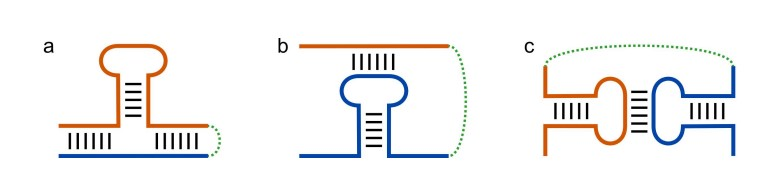
\includegraphics[width=0.9\linewidth]{concat}
		\centering
		\caption{a) Pattern that can be predicated by Concatenation b)Kissing stem-loop c) kissing hairpin interaction. The blue and orange are the two different RNA's and the dotted green is the linker , black lines represents the base pairs. } 
		\label{fig:concat}
	\end{figure}
	
	The energy for the concatenation approach, as we have linker here it becomes as a one interior loop.\\
	
	\subsection{Accessibility}
	Concatenation approaches cannot predict the structures which contains pseudoknots. To overcome the drawback of concatenation approach, Accessibility approaches has been introduced. The main aim of this approach is to ensemble properties of the single sequences that are necessary for the interaction. Tools like RNAup and IntaRNA can be used to predict such approaches. Here we have to neglect the intra molecular structure before the intermolecular interaction is formed. In order to form a stable interaction of intermolecular base pairs, the intra molecular base pairs has to be opened /broken. \\
	
	The accessibility-incorporating interaction scorings
	are computed and stored in table $I$. A non-zero entry $I^{i,k}_{j,l}$
	represents the combined scoring for an interaction of
	$S^1_{i..k}$ with $\overleftarrow{S^2_{j..l}}$ with
	left/right most base pairs $(S^1_i,\overleftarrow{S^2_j})$/$(S^1_k,\overleftarrow{S^2_l})$, respectively.\\


	\begin{equation}
	\label{eq:4}
	I^{i, k}_{j, l} = max \begin{cases}
	(E^{bp} \cdot D^{i, k}_{j, l} +ED^{1}_{i,k} +ED^{2}_{j, l}) & : \text{if } D^{i, k}_{j, l} > 0  ,\\-\infty & :\text{otherwise}
	\end{cases}
	\end{equation}
	
	 Where $ED^{1}_{i,k} = - RT \cdot \log(P^{u1}_{i,k}),\\ ED^{2}_{j, l} =  - RT \cdot \log(P^{u2}_{j, l})$\\
	 
	The maximal number of base pairs $D^{i,k}_{j,l}$ for all interaction sites are computed using hybrid approach. Then the  unpaired probabilities $P^{u1}$ and $P^{u2}$ are tabularized for both sequences $S^1$ and $\overleftarrow{S^2}$, respectively using mcckaskill approach.\\
	
	\begin{figure}[h]
		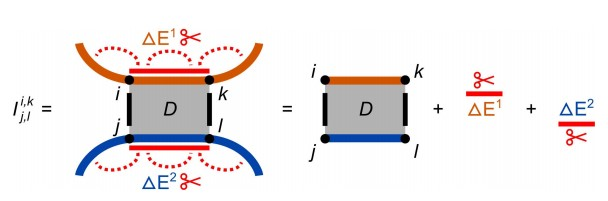
\includegraphics[width=0.9\linewidth]{access}
		\centering
		\caption{ Depiction how accessibility-based approaches score an interaction of two RNAs $S1$ and $S2$ in orange and blue respectively} 
		\label{fig:access}
	\end{figure}
	
	To further simplify the recursions, we use dedicated calculations for the duplex energy and the overall interaction energy. This is a 4-d matrix, in which $D^{i, k}_{j, l}$ provides the the duplex energy of the interacting sites ~\ref{eq:5}. 
	The first case represents the initiation of a new interaction that covers only the intermolecular base pair (i,j), second case is the extension of already computed interaction of  $S^1_{p..k}, \overleftarrow{S^2_{q..l}}$ with a new base pair $(i,j)$ and the third case is used if base pairs cannot be formed.\\
	
	\begin{equation}
	\label{eq:5}
	D^{i, k}_{j, l} = max \begin{cases}
	1 & : \text{if } S^1_i, \overleftarrow{S_j^2} \text{ compl.}, i = k, j = l \\ \underset{\substack{i<p\leq k,\;j<q\\leq l}}{\max}\left( 1 + D_{q, l}^{p, k} \right) &: \text{if } S^1_i, \overleftarrow{S^2_j} \text{ compl.}, i < k, j < l ,\\ -\infty & : \text{otherwise}
	\end{cases}
	\end{equation}
	
	The energy of accessibility approach, we will no break. Approaches like RNAup and IntaRNA use precalculated ED values for all possible interaction regions. They gives us how much energy is needed to free of intramolecular base pairs. The main drawback of accessibility approach is, it can handle only one crossing blocks. These approaches cannot be modelled correctly for the double kissing hairpin interaction which has more than one crossing blocks of interaction.\\
	
	
	\subsection{Comparison with approaches}
	In this subsection, we will see the comparison between the approaches for few interaction pattern. Below table ~\ref{table:1} gives the overview for which interaction pattern , the approaches can be used. \\
	
	\begin{table}[H]
		\begin{spacing}{0.5}
	  \caption{ Comparison of RNA-RNA interaction prediction approaches for different figures}
	\label{table:1}
	\begin{tabularx}{\hsize}{l*{7}{L}}
		\toprule
		\multicolumn{8}{c}{\textbf{Comparison of RRI approaches}}\\  
		\midrule
		& \multicolumn{3}{c}{\textbf{RRI pattern}} 
		&	\multicolumn{4}{c}{\textbf{RRI prediction approaches}}\\
		\cmidrule(r){2-4}  \cmidrule(l){5-8}
		No. & Figures & RRI description& No.of blocks& \rotatebox[origin=c]{90} {Hybrid}  &\rotatebox[origin=c]{90}{General}  &\rotatebox[origin=c]{90}{Concatenation}  &\rotatebox[origin=c]{90}{Accessibility} \\
	 	\midrule
	 	\addlinespace[0.5cm]
		1& ~\ref{fig:rnahybrid}&Full duplex structure&1 &yes &yes &yes &yes\\
		\addlinespace[1cm]
		2& ~\ref{fig:concat} (a)& Nested joint structure (without pseduknots) &2 & no &yes &yes &yes \\
		\addlinespace[1cm]
		3 & ~\ref{fig:concat} (b)& Kissing stem  &1 & no &yes &no &yes \\
		\addlinespace[1cm]
		4 & ~\ref{fig:concat} (c)& Kissing hairpin  &1 & no &yes &no &yes \\
		\addlinespace[1cm]
		5 & ~\ref{fig:doublekiss}&Double kissing hairpin  &2 &no &yes &no &no\\
		\addlinespace[1cm]
		\bottomrule
		\end{tabularx}
	\end{spacing}
   \end{table}

	We could conclude that the accessibility based approach is the best approach for single site RNA-RNA interaction. As, they can't predict the multisite RRI because in IntaRNA model, we remove the base pairs while predicting, when they are no intramolecular base pairs are in between, it is considered to be a wrong model (ie., double kissing hairpin loop interaction).  To handle two or multi crossing blocks of interaction, we are introducing multisite accessibility based approach. The Multi-site RRI optimization is based on single-site IntaRNA predictions. Hence, we are going for the multisite accessibility based approach in the next chapter.\\

		
		
		
	\chapter{Multisite Accessibility Based  }
	\chapter{Results}
	\chapter{Discussion and conclusion}
	
	
	\bibliographystyle{plainnat}
	\bibliography{ref}

	
\end{document}